\section{Theory}\label{sec:WBoson_Theory}


INTRO PARRAGRAPH MISSING


\subsection{History of weak theory}

In the early 20th century, quantum mechanics was the standard framework of atomic physics but certain processes such as the $\beta$ decay, discovered by Ernest Rutherford in 1899~\cite{RutherfordBetaDecay}, were not fully understood yet. At the time, the $\beta$ decay was characterized by the process $A_{i}\rightarrow{A_{f}+e^{-}}$, where an initial nucleus $A_{i}$ decays into another nucleus $A_{f}$ emitting an electron during the process. In order to conserve energy, the electron is required to have a fixed kinetic energy, but James Chadwick observed in 1914 that the $\beta$ rays produced a continuos energy spectrum~\cite{BetaDecay_1,BetaDecay_2} in disagreement with was expected. As a way to solve the problem of the continuous $\beta$ decay spectrum, Wolgang Pauli proposed in 1930 the existence of a new particle~\cite{Neutrino_1,Neutrino_2}. Pauli named his particle initially the neutron but later renamed it to the neutrino after the discovery of a new electrically neutral particle inside the ${}_{7}^{14}\mathrm{Ni}$ nucleus by Chadwick in 1932~\cite{Neutron}. Pauli described the neutrino as a neutral fermion with mass close to zero and spin $1/2$ capable of penetrating matter deeper than photons~\cite{Neutrino_1}.

Enrico Fermi, after attending the 7th Solvay conference where the discovery of the neutron as well as Pauli's neutrino were presented, proposed a new theory to explain the $\beta$ decay~\cite{FermiWeakTheory_1}. Fermi's theory defined the $\beta$ decay as a process in which the neutron decays to a proton, emitting an electron and a neutrino. Fermi formulated his theory using an analogous approach as in Quantum Electrodynamics (QED) by proposing the following lagrangian for $\beta$ decay~\cite{FermiWeakTheory_2}:

\begin{equation}
L_{\beta}=G_{F}\left(\bar{u}_{p}\gamma_{\mu}u_{n}\right)\left(\bar{u}_{e}\gamma^{\mu}u_{\nu}\right)
\end{equation}

where $u$ is the Dirac spinor of each particle, $\gamma_{\mu}$ is the Dirac matrix and $G_{F}$ is the Fermi coupling constant. Fermi's theory of weak interations assumed the same conservation rules as QED, including the symmetry under reflection in space~\cite{FermiWeakTheory_2}. A system that is invariant under reflections conserve a quantity called parity which includes an intrinsic component called spin and a spatial component depending on the angular momentum of the particle.

In the upcoming years, the physicists Tsung Dao Lee and Chen Ning Yang started to doubt the conservation of weak parity after not finding any experimental evidence so far~\cite{LeeYang}. In an attempt to test the conservation of parity in weak interactions, Lee and Yang proposed in 1956 to study the $\beta$ decays of Cobalt (${}^{60}$Co) and measure the projection of the momemtum of electrons along the spin axis of the Cobalt nucleus~\cite{LeeYang}. If the decay process conserves parity then electrons would be produced in all directions. The experiment to test the conservation of weak parity was realized by Chien-Shiung Wu in 1957. The results of Wu's research showed that electrons were preferentially produced in the opposite direction to the Cobalt spin~\cite{WuParityViolation}, which meant that parity was not conserved in weak interactions.

Apart from parity, one can also associate a helicity to particles. The particle's helicity is considered right-handed if the direction of the particle's momemtum and spin are the same, and left-handed otherwise. In 1958, Goldhaber, Grodzins and Sunyar measured the neutrino helicity at Brookhaven National Laboratory (BNL) and discovered that neutrinos were always left-handed and antineutrinos were right-handed~\cite{NeutrinoHelicity}. As a consequence of the discovery of parity violation and the neutrino helicity, Lee and Yang modified Fermi's weak theory and introduced an axial vector term, giving rise to the V-A (vector-axial) theory of weak interactions. Even though parity (P) and charge conjugation (C) (transforms particles into their antiparticles) were violated separately, it was assumed that the combined CP operation was still conserved by the weak force.

The assumption of the conservation of CP did not last long. An experiment performed at BNL by James Christenson, James Cronin, Val Fitch and Rene Turlay~\cite{KMeson} in 1964 concluded that the long-lived $K_{L}$ meson (CP=-1) was able to decay to two pions (CP=+1) violating CP in the process. To explain the CP violation in weak theory, Makoto Kobayashi and Toshihide Maskawa~\cite{CKMMatrix} extended the formulation of the Cabibbo matrix to include three generation of quarks and a CP-violating phase term. The Cabibbo matrix was originally computed by Nicola Cabibbo~\cite{CabibboMatrix} including four quarks to explain the different amplitudes observed between the up, down and strange quark transitions. The development of the Cabibbo, Kobayashi and Maskawa (CKM) matrix led to the prediction of the bottom and top quarks, discovered later in 1977~\cite{BottomQuarkDiscovery} and 1995~\cite{TopQuarkDiscovery}, respectively.

Following Paul Dirac's formulation of QED~\cite{DiracQED}, Sheldon Glashow~\cite{Glashow:1959wxa}, Steven Weinberg~\cite{Weinberg:1967tq} and Abdus Salam~\cite{Salam:1968rm} managed in 1968 to build a gauge-invariant unified theory of the electromagnetic and weak interactions, for which they were awarded the Nobel Prize in Physics in 1979~\cite{Nobel1979}. In order to make the electroweak theory symmetric under local phase transformations, it required the presence of four spin-1 massless bosons: two electricaly charged particles called $W^{\pm}$ bosons and two neutral particles corresponding to the Z boson and photon. But since weak interactions are short range, the weak force has to be mediated by massive bosons. The addition of mass to the bosons was realized after introducing the spontaneous local breaking of the underlying SU(2) symmetry through the Higgs mechanism~\cite{HiggsMechanism_1,HiggsMechanism_2}. In the following years, Gerardus't Hooft and Martinus Veltman managed to renormalize the electroweak theory~\cite{Renormalization_1,Renormalization_2}, allowing to calculate more precisely the theoretical masses of the weak bosons.

The experimental study of weak bosons would require the development of new particle acceleration technologies. In 1976, Carlo Rubbia, Peter McIntyre and David Cline suggested to transform CERN's circular proton accelarator called Super Proton Synchroton (SPS) into a proton-antiproton collider (Sp$\bar{\mathrm{p}}$S)~\cite{SppS}. The upgrade to Sp$\bar{\mathrm{p}}$S was made possible thanks to the stochastic cooling technology invented by Simon Van der Meer~\cite{StochasticCooling} in 1972, which allowed to cool down and collect antiprotons. Several experiments, named Underground Area (UA), were built to study the proton-antiproton collisions at the Sp$\bar{\mathrm{p}}$S. The UA1 and UA2 collaborations discovered the W boson~\cite{W_UA1,W_UA2} in 1983 after reporting the observation of electrons with large transverse energy and the presence of missing energy in p$\bar{\mathrm{p}}$ collisions at $\sqrt{s}=540$~\GeV. And few months later, both collaborations also reported the discovery of the Z boson in the dilepton decay channel~\cite{Z_UA1,Z_UA2}. These outstanding discoveries convinced the Swedish Academy of Science to award in 1984 the Nobel Prize in Physics to Rubbia and Van der Meer for their contributions to the Sp$\bar{\mathrm{p}}$S program~\cite{Nobel1984}.

After the major success of the Sp$\bar{\mathrm{p}}$S project, CERN constructed in 1983 a new lepton circular collider called the Large Electron-Positron (LEP) collider~\cite{LEP}. LEP was designed to accelerate electrons and positrons to an energy of half the {\PZ} boson mass (45~\GeV) in order to perform precision measurements of the {\PZ} boson lineshape. Furthermore, a precise measurements of the {\PW} mass~\cite{WMass_D0} was later performed by the experiments in the Fermi National Accelarator Laboratory (FNAL). The FNAL analyzed data collected between 1983 and 2011 from the Tevatron~\cite{Tevatron}, a proton-antiproton synchrotron collider that operated at energies up to 1~\TeV.

The succesful programs of LEP and Tevatron produced the most precise measurements of the properties of the electroweak theory, but there was still a missing piece to complete the picture, the Higgs boson. The discovery of the Higgs boson was finally achieved in 2012 by the CMS~\cite{HiggsBoson_CMS} and ATLAS~\cite{HiggsBoson_ATLAS} collaborations at the Large Hadron Collider (LHC).


\subsection{Electroweak theory}

The interactions between elementary particles mediated by the weak and electromagnetic forces are described in the Standard Model using the electroweak theory developed by Glashow, Weinberg and Salam~\cite{Glashow:1959wxa,Weinberg:1967tq,Salam:1968rm}. The unification of these two fundamental forces of nature is accomplished mathematically using a non-abelian $SU(2) \times U(1)_{Y}$ gauge theory. The electroweak theory requires four massless gauge bosons: three bosons with weak isospin (called $W_{1}$, $W_{2}$ and $W_{3})$ from $SU(2)$ and one boson (named $B$) with weak hypercharge from $U(1)_{Y}$.

Since weak bosons have mass, a full description of the electroweak interactions requires the inclusion of massive vector bosons. The problem is that one can not naively add a mass term of the form $m^{2}W^{\mu}W_{\mu}$ into the electroweak lagrangian since this would break gauge invariance making the theory divergent. Thus, this issue is instead solved by spontaneously breaking the $SU(2) \times U(1)_{Y}$ electroweak symmetry into a $U(1)_{EM}$ symmetry using the Higgs mechanism~\cite{HiggsMechanism_1,HiggsMechanism_2}. The overall idea is that the electroweak gauge bosons couple to a scalar field called the Higgs field which is present in all space. When the Higgs field induces a spontaneous breaking of the gauge symmetry, the Higgs field is splitted into one dynamic part corresponding to the Higgs boson, and another constant part called the vacuum expectation value (VEV). The symmetry breaking of $SU(2) \times U(1)_{Y}$ to $U(1)_{em}$ generates three massless Goldstone bosons. The goldstone bosons are then absorbed by the electroweak gauge bosons producing the $\PW^{+}$, $\PW^{-}$ and {\PZ} bosons with masses proportional to the VEV, while the photon remains massless. The $\PW^{\pm}$, {\PZ} and $\gamma$ bosons are correlated with the $W_{1}, W_{2}, W_{3}$ and $B$ gauge bosons in the following way:

\begin{equation}
  \begin{split}
    W^{\pm} & = \frac{1}{\sqrt{2}}\left(W_{1} \pm W_{2}\right) \\
    \begin{pmatrix} Z \\ \gamma \end{pmatrix} & = \begin{pmatrix} \mathrm{cos}{\theta_{W}} & \mathrm{sin}{\theta_{W}} \\ -\mathrm{sin}{\theta_{W}} & \mathrm{cos}{\theta_{W}} \end{pmatrix} \begin{pmatrix} B \\ W_{3} \end{pmatrix}
  \end{split}
  \label{eq:ElectroWeakBosons}
\end{equation}

where $\theta_{W}$ represents the weak mixing angle. In addition, the quarks acquire mass through the Yukawa interaction with the Higgs field. Since the quark weak eigenstates are not the same as their mass eigenstates, weak interactions can induce a transition from a up-like quark ($u, c, t$) to a down-like quark ($d, s, b$). The strength of the quark flavour mixing in weak deacays is parameterized by the CKM matrix $\mathrm{V}_\mathrm{CMK}$ via:

\begin{equation}
\begin{pmatrix} d' \\ s' \\ b' \end{pmatrix} = \begin{pmatrix} \mathrm{V}_{ud} & \mathrm{V}_{us} & \mathrm{V}_{ub} \\ \mathrm{V}_{cd} & \mathrm{V}_{cs} & \mathrm{V}_{cb} \\ \mathrm{V}_{td} & \mathrm{V}_{ts} & \mathrm{V}_{tb} \\ \end{pmatrix}\begin{pmatrix} d \\ s \\ b \end{pmatrix}
\end{equation}

where ($d'$, $s'$, $b'$) are the down-like quark weak eigenstates and ($d$, $s$, $b$) are the corresponding mass eigenstates. The latest values of the CKM matrix elements are~\cite{PDG}:

\begin{equation}
\mathrm{V}^\mathrm{CKM} = \begin{pmatrix} 0.97417 & 0.2248 & 0.00409 \\ 0.220 & 0.995 & 0.0405 \\ 0.0082 & 0.04 & 1.009 \\ \end{pmatrix}
\end{equation}

The lagrangian of the electroweak theory includes several components that describes the interactions between the fermions, electroweak bosons and the Higgs boson. In the case of the {\PZ} boson, the term of the lagrangian that represents the interactions between fermions and neutral charged electroweak bosons is:

\begin{equation}
  \begin{split}
    L_{NC} &= {\alpha_{em}{\theta_{W}}}\sum_{fermions}\bar{f}\gamma^{\mu}A_{\mu}f + \frac{g}{\mathrm{cos}{\theta_{W}}}\sum_{fermions}\bar{f}\gamma^{\mu}\frac{\left(g^{f}_{v}-g^{f}_{a}\gamma^{5}\right)}{2}Z_{\mu}f
  \end{split}
  \label{eq:NeutralCurrent}
\end{equation}

where $g$ is the coupling constant of $SU(2)_{L}$, $f$ is the Dirac spinors of fermions, $A_{\mu}$ is the electromagnetic field, and $g^{f}_{v}$ ($g^{f}_{a}$) is the fermion vector (axial) weak coupling constants. \eq{eq:NeutralCurrent} specify that the {\PZ} bosons and photons conserve flavour always decaying into a fermion and its corresponding antifermion. Even though photons do not distinguish the helicity of particles, the {\PZ} boson couplings are different for left- and right-handed fermions.

Furthermore, the component of the lagrangian that represents the interaction between the {\PW} bosons and the fermions is given by:

\begin{equation}
  \begin{split}
    L_{CC} &= \frac{g}{2\sqrt{2}}\left(\left(\bar{u}, \bar{c}, \bar{t}\right)_{R}W^{+}_{\mu}\gamma^{\mu}\mathrm{V}^{\mathrm{CKM}}\begin{pmatrix} d_{L} \\ s_{L} \\ b_{L} \\ \end{pmatrix} + \left(\bar{\nu}_{e}, \bar{\nu}_{\mu}, \bar{\nu}_{\tau}\right)_{R}W^{+}_{\mu}\gamma{\mu}\begin{pmatrix} e^{-}_{L} \\ \mu^{-}_{L} \\ \tau^{-}_{L} \\ \end{pmatrix}\right)
  \end{split}
\end{equation}

where $f_{L}$ correspond to left-handed fermions and $\bar{f}_{R}$ represents right-handed antifermions. Thus, {\PW} bosons only couple to right-handed antifermions and left-handed fermions organized in pairs of lepton-neutrino or quark-antiquark, where the electric charge of the of particles differ by one unit. Since the top quark mass (178~\GeV) is larger than the {\PW} boson mass (80~\GeV), the {\PW} boson can not decay to a top quark. \fig{dia:WDecays} shows the possible decays of {\PW} bosons to fermions. The measured values of the mass, width and couplings of weak vector bosons are summarized in \tab{tab:ElectroweakParameters}.

\begin{figure}[htbp]
  \vspace{10mm}
  \begin{center}
    \subfloat{
      \begin{fmffile}{WPlus}
        \begin{fmfgraph*}(120,70)
          \fmfleft{v1}
          \fmfright{o1,o2}
          \fmflabel{${\nu}_{e}, {\nu}_{\mu}, {\nu}_{\tau}, d', s'$}{o1}
          \fmflabel{$e^{+}, \mu^{+}, \tau^{+}, \bar{u}, \bar{c}$}{o2}
          \fmf{fermion}{o2,v2,o1}
          \fmf{boson,label=$\text{W}^{+}$,label.side=right}{v1,v2}
        \end{fmfgraph*}
      \end{fmffile}
    }
    \hspace*{2cm}
    \subfloat{
      \begin{fmffile}{WMinus}
        \begin{fmfgraph*}(120,70)
          \fmfleft{v1}
          \fmfright{o2,o1}
          \fmflabel{$e^{-}, \mu^{-}, \tau^{-}, u, c$}{o1}
          \fmflabel{$\bar{\nu}_{e}, \bar{\nu}_{\mu}, \bar{\nu}_{\tau}, \bar{d}', \bar{s}'$}{o2}
          \fmf{fermion}{o2,v2,o1}
          \fmf{boson,label=$\text{W}^{-}$,label.side=right}{v1,v2}
        \end{fmfgraph*}
      \end{fmffile}
    }
  \end{center}
  \caption{Feynman diagram of the decay modes of $\PW^{+}$ (left) and $\PW^{-}$ (right) bosons to fermions.}
  \label{dia:WDecays}
\end{figure}

\begin{table}[htbp]
  \begin{center}
    \begin{tabular}{ c c c }
    Variable & Description & Value \\ \hline
    $M_{\PW}$ & {\PW} boson mass & $80.385 \pm 0.015$~\GeV \\
    $\Gamma_{\PW}$ & {\PW} boson width & $2.085 \pm 0.042$~\GeV \\
    $\mathrm{BR}\left(\PW\rightarrow{\ell\nu}\right)$ & Branching fraction of {\PW} boson semileptonic decays & $\left(10.86 \pm 0.09\right)\%$ \\
    $\mathrm{BR}\left(\PW\rightarrow{q\bar{q}'}\right)$ & Branching fraction of {\PW} boson hadronic decays & $\left(67.41 \pm 0.27\right)\%$ \\
    \hline
    $M_{\PZ}$ & {\PZ} boson mass & $91.1876 \pm 0.0021$~\GeV \\
    $\Gamma_{\PZ}$ & {\PZ} boson width & $2.4952 \pm 0.0023$~\GeV \\
    $\mathrm{BR}\left(\PZ\rightarrow{\ell^{+}\ell^{-}}\right)$ & Branching fraction of {\PZ} boson charged-lepton decays & $\left(3.3658 \pm 0.0023\right)\%$ \\
    $\mathrm{BR}\left(\PZ\rightarrow{\nu\bar{\nu}}\right)$ & Branching fraction of {\PZ} boson neutrino decays & $\left(20.00 \pm 0.06\right)\%$ \\
    $\mathrm{BR}\left(\PZ\rightarrow{q\bar{q}}\right)$ & Branching fraction of {\PZ} boson hadronic decays & $\left(69.91 \pm 0.06\right)\%$
    \end{tabular}
  \end{center}
  \label{tab:ElectroweakParameters}
  \caption{Experimental values of the mass, width and branching fractions of weak bosons extracted from the PDG~\cite{PDG}.}
\end{table}


\subsection{Hadron collisions at the LHC}

Hadrons are not elementary particules due to their internal structure composed of partons (i.e. quarks and gluons). The production of particles in hadronic collisions depends on the evolution of the partons inside the hadrons and the parton momentum transfer during the hard scattering. In this thesis, the production of {\PW} bosons is determined from collisions of protons against Lead ions (\pPb), so we need to take into account the interplay between protons and Pb nuclei.

Protons can be described as a collection of three valence quarks: one down quark and two up quarks. The quantum properties of the proton, such as the electric charge or spin, are derived from the valence quarks. The interaction between valence quarks is mediated by the exchange of gluons. Gluons inside the hadrons can also produce quark-antiquark pairs and other gluons through self interactions. The quark-antiquark pairs produced inside the hadron are called sea quarks and only exist virtually. The gluons and sea quarks do not contribute to the quantum numbers of hadrons but they play a key role in the interaction of hadrons with other particles.

Since the strength of the strong interactions decreases with energy,  the partons can be considered effectively free within the proton during high energy collisions. In this case, each parton carries a fraction of the proton's total momemtum, represented by the quantity called Bjorken x~\cite{BjorkenX} (labelled simply as x), given by:

\begin{equation}
p_{parton} = xp_{proton}
\end{equation}

The parton distribution functions (PDF) describes the probability that a parton carries a given fraction of the proton's momemtum. The PDFs can not be currently calculated due to the nonperturbative nature of QCD, but they can be constrained from fits to experimental data due to the factorization theorem.

The factorization theorem indicates that the cross section of a given process in hadronic collisions can be factorized, in all orders of the perturbative expasion, into a partonic cross section and the  nonperturvative PDFs of the incoming hadrons. The partonic cross section can be derived using perturbative QCD regardless of the incoming hadron while the PDFs can be determined from global fits to the data since they are universal (i.e. the PDFs are independent of the initial process). The hadronic cross section in a given final state can be expressed at leading order, using the factorization theorem, as:

\begin{equation}
\sigma_{h1,h2} = \sum_{f1,f2=(q,\bar{q},g)}\int_{0}^{1}dx_{1}dx_{2}f_{1}^{h1}\left(x_{1},Q^{2}\right)f_{2}^{h2}\left(x_{2},Q^{2}\right)\hat{\sigma}_{f_{1}f_{2}}
\label{eq:FactTheorem}
\end{equation}

where $Q^{2}$ is the momentum scale, $f\left(x,Q^{2}\right)$ is the PDF, and $\hat{\sigma}$ represents the partonic cross section. The $Q^{2}$ scale dependence of the PDFs is described by the parton evolution equations developed by Dokshiftzer, Gribov, Lipatov, Altarelli and Parisi (DGLAP)~\cite{DGLAP_1,DGLAP_2,DGLAP_3}. 

In the DGLAP formalism, the PDFs can be expressed in terms of kernels $P_{q_{1}q_{2}}$ (called splitting functions), and the evolution equations of the quark $q$ and gluon $g$ densities can be written as:

\begin{equation}
  \begin{alignedat}{1}
    \frac{d}{dt}q_{i}\left(x,t\right) &= \frac{\alpha_{s}\left(Q\right)}{2\pi}\left[q_{i}\circledast{P_{qq}} + g_{i}\circledast{P_{qg}}\right] \\
    \frac{d}{dt}g\left(x,t\right) &= \frac{\alpha_{s}\left(Q\right)}{2\pi}\left[\sum_{i}\left(q_{i}+\bar{q}_{i}\right)\circledast{P_{gq}} + g_{i}\circledast{P_{gg}}\right] \\
    \left[q\circledast{P}\right] &= \int_{x}^{1}d\epsilon\frac{(q\left(\epsilon,t\right)}{\epsilon}\times{P\left(\frac{x}{\epsilon}\right)}
  \end{alignedat}
  \label{eq:DGLAP}
\end{equation}

where $t \propto \mathrm{Log}\left(Q^{2}\right)$, and $P_{q_{1}q_{2}}$ is the probability of finding a parton $q_{1}$ in another parton $q_{2}$. In other words, the DGLAP evolution equations state that the PDF of a given parton $q$ at an x value is determined from the contribution of all the partons at higher momentum fraction considering their probability of decaying into the parton $q$.

From the definition of the PDFs, one can also formulate a set of structure functions defined as:

\begin{equation}
F^{p}_{2}\left(x\right) = \sum_{f}e_{f}^{2}f\left(x,Q^{2}\right)x
\end{equation}

where $e_{f}$ is the electric charge of a given fermion $f$. The structure functions were extensively measured in Deep-Inelastic Scattering (DIS) collisions at the Hadron-Elektron-Ringanlage (HERA) accelarator by the ZEUS and H1 collaborations. The measurements of the $F_{2}$ structure function performed by the ZEUS collaboration~\cite{HERAStrucFunc} at HERA are shown in \fig{fig:HERAStrucFunc}.

\begin{figure}[htbp]
 \begin{center}
  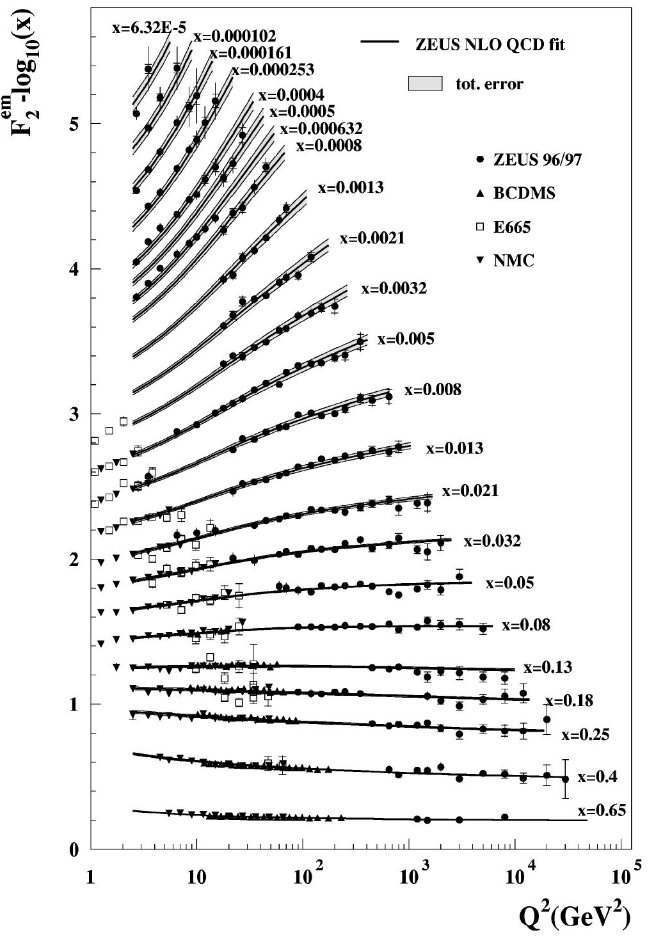
\includegraphics[width=0.5\textwidth]{Figures/WBoson/Theory/Structure_Function.png}
 \end{center}
\caption{NLO QCD fits to the to the ZEUS $F_{2}$ structure function data from 1996, 1997 and proton fixed-target at HERA. The error bands of the fit represent the total experimental uncertainty from both correlated and uncorrelated sources. Figure taken from Ref.~\cite{HERAStrucFunc}}
 \label{fig:HERAStrucFunc}
\end{figure}

The DIS process consists in the inelastic scattering of electrons off protons as presented in \fig{dia:DIS}. In the DIS process, the momentum transferred from the electron to the proton is defined as $Q^{2} = -q^{2} = -\left(k - k'\right)^{2}$ and the corresponding Bjorken x fraction is $x = {Q^{2}}\big/{2\left(p^{h}_{in}.q\right)}$. Even though DIS experiments were not able to probe the gluons directly, the DIS data showed that valence quarks did only carry half of the proton momentum been the rest carried by the gluons.

\begin{figure}[htbp]
  \vspace{10mm}
  \begin{center}
  \begin{fmffile}{DIS}
    \begin{fmfgraph*}(160,100)
      \fmfleft{ip,il}
      \fmfright{x1,x2,x3,o1,o2,o3,o4,ol}
      \fmfset{arrow_len}{10}
      % lepton
      \fmflabel{$\text{e}^-$}{il}
      \fmflabel{$\text{e}^-$}{ol}
      \fmf{fermion,label=$k$, label.side=left}{il,vl}
      \fmf{fermion,label=$k'$,label.side=left}{vl,ol}
      \fmf{phantom,tension=0.6}{vl,vp}
      % proton
      \fmfv{l=$\text{p}^+$,l.a=-160}{ip} % l.a = label.angle
      \fmf{phantom,tension=1}{ip,vp,x1}
      \fmffreeze
      \fmfi{fermion}{vpath (__ip,__vp) scaled 1.01}
      \fmfi{fermion,label=$p$,label.side=left}
                    {vpath (__ip,__vp) scaled 1.01 shifted (-1.4, 6)}
      \fmfi{fermion}{vpath (__ip,__vp) scaled 1.01 shifted ( 1.4,-6)}
      \fmfblob{25}{vp}
      % X
      \fmfv{l=\mybrace{40} $X$,l.a=10}{x2}
      \fmf{fermion}{vp,x1}
      \fmf{phantom}{vp,x2} % to help \fmfi
      \fmfi{fermion}{vpath (__vp,__x2) scaled 0.98 shifted (0,2.2)}
      \fmffreeze
      % photon
      \fmf{photon,label=\vspace{-4pt}\hspace{5pt}{$q$},label.side=left}{vl,v}
      % parton
      \fmf{fermion,label=$xp$,label.side=left}{vp,v}
      \fmf{fermion}{v,o2}
    \end{fmfgraph*}
  \end{fmffile}
  \end{center}
  \caption{Feynman diagram of deep inelastic scattering of electrons against protons}
  \label{dia:DIS}
\end{figure}

Another important process that takes place in hadron colliders is the Drell-Yan (DY) production.  In the DY process a quark from one hadron and an antiquark from another hadron annihilate into a virtual photon ($\gamma^{*}$) or {\PZ} boson which then decays to a pair of leptons as shown in \fig{dia:DY}. Drell-Yan production is used to constrain the quark PDFs in a wide range of momentum fraction x depending on the invariant mass of the dilepton pair. In addition, the Drell-Yan process also contributes to the background of the {\PW} boson production when one the DY final state leptons is generated outside of the detector acceptance.

\begin{figure}[htbp]
  \vspace{10mm}
  \begin{center}
\begin{fmffile}{DY}
  \begin{fmfgraph*}(160,160)
    \fmfleft{i1,iq,i2,ip,i3}
    \fmfright{y1,y2,y3,o1,f1,o2,o3,o4,f2,o5,x3,x2,x1}
    \fmfset{arrow_len}{10}
    % skeleton
    \fmf{phantom,tension=0.48}{vq,vp}
    \fmf{phantom}{ip,vp,x1}
    \fmf{phantom}{iq,vq,y1}
    \fmffreeze
    % parton
    \fmfv{l=$x_1p_1$,l.a=-90,l.d=22}{vp} % cheat: actually a line label
    \fmfv{l=$x_2p_2$,l.a=90,l.d=22}{vq} % cheat: actually a line label
    \fmf{fermion,tension=1.6}{vp,v}
    \fmf{fermion,tension=1.6}{v,vq}
    % hard process
    \fmfshift{20 right}{f1,f2}
    \fmfv{l=$\bar{f}$}{f1}
    \fmfv{l=$f$}{f2}
    \fmf{boson,tension=2,label=$\text{Z}^0/\gamma^*$,label.side=left}{v,vf}
    \fmf{fermion,tension=2}{f1,vf,f2}
    % proton 1
    \fmfv{l=${h}_{A}$,l.a=180,l.d=10}{ip}
    \fmf{phantom}{ip,vp}
    \fmfi{fermion,l=$p_1$,l.s=left,l.d=8}
                  {vpath (__ip,__vp) scaled 1.01 shifted (-2.4, 6)}
    \fmfi{fermion}{vpath (__ip,__vp) scaled 1.01 shifted (-2.4, 0)}
    \fmfi{fermion}{vpath (__ip,__vp) scaled 1.01 shifted (-2.4,-6)}
    % proton 2
    \fmfv{l=${h}_{B}$,l.a=180,l.d=10}{iq}
    \fmf{phantom}{iq,vq}
    \fmfi{fermion}{vpath (__iq,__vq) scaled 1.01 shifted (-2.4, 6)}
    \fmfi{fermion}{vpath (__iq,__vq) scaled 1.01 shifted (-2.4, 0)}
    \fmfi{fermion,l=$p_2$,l.s=right,l.d=8}
                  {vpath (__iq,__vq) scaled 1.01 shifted (-2.4,-6)}
    % X 2
    \fmfshift{25 left}{x1}
    \fmfshift{20 left}{x2,x3}
    \fmf{phantom}{vp,x1} % to help \fmfi
    \fmf{phantom}{vp,x2} % to help \fmfi
    \fmf{phantom}{vp,x3} % to help \fmfi
    \fmfi{fermion}{vpath (__vp,__x1) scaled 1.0 shifted ( 0.0, 2.0)}
    \fmfi{fermion}{vpath (__vp,__x2) scaled 1.0 shifted ( 0.0, 0.0)}
    \fmfi{fermion}{vpath (__vp,__x3) scaled 1.0 shifted ( 0.0,-2.0)}
    \fmfblob{25}{vp}
    % X 2
    \fmfshift{25 left}{y1}
    \fmfshift{20 left}{y2,y3}
    \fmf{phantom}{vq,y1} % to help \fmfi
    \fmf{phantom}{vq,y2} % to help \fmfi
    \fmf{phantom}{vq,y3} % to help \fmfi
    \fmfi{fermion}{vpath (__vq,__y1) scaled 1.0 shifted ( 0.0,-2.0)}
    \fmfi{fermion}{vpath (__vq,__y2) scaled 1.0 shifted ( 0.0, 0.0)}
    \fmfi{fermion}{vpath (__vq,__y3) scaled 1.0 shifted ( 0.0, 2.0)}
    \fmfblob{25}{vq}
  \end{fmfgraph*}
\end{fmffile}
  \end{center}
  \caption{Feynman diagram of neutral charged Drell-Yan process}
  \label{dia:DY}
\end{figure}


We have considered until now only the structure of protons, but the nuclear enviroment of ions can also impact the production of particles. Pb ions are composed of 82 protons and 126 neutrons. The neutron PDF can be derived from the proton PDF using isospin symmetry (i.e. by exchanging the up and down quark PDFs), while assuming the same gluon PDF as in the proton. If no nuclear modifications are expected, protons and neutrons should then behave as free particles inside the nucleus, and one could simply sum the PDFs of the protons and neutrons scaled accordingly. In this case, the ratio of the PDF of protons bounded in the nucleus (nuclear PDF) over the free-proton PDF should be one.

To determine the nuclear modifications, the heavy ion measurements were first compared to results using deuterium. The European Muon Collaboration (EMC) measured the structure function of DIS in iron and deuterium targets between 1977 and 1988, and observed a depletion of the iron PDFs relative to the deuterium PDFs at $x>0.2$ (EMC region)~\cite{EMCStrucFunc_1} and at $x<0.01$ (shadowing region)~\cite{EMCStrucFunc_2}. Subsequent results found an enhancement at the intermediate region $0.01 < x < 0.2$ (antishadowing region)~\cite{NMCStrucFunc}. Since current heavy ion data is more limited than data from proton collisions, the global fits of the nuclear PDFs are less accurate than the proton PDFs.

\subsection{PDF global fits}

The parton distribution functions can not be currently determined from first principles due to the nonperturbative behaviour of the strong interactions. Nevertheless, their depencence on x can be derived by fitting observables (e.g. structure functions or asymmetries) to experimental data from different processes since PDFs do not depend on the initial hard scattering. The $Q^{2}$ dependence of the PDFs is determined using the DGLAP evolution equations. The most common processes used to constrain the PDFs correspond to Drell-Yan, DIS, vector boson and jet production, which have been measured by various experiments including data from HERA, SLAC and LHC.

There are several proton PDFs currently available. One of the most commonly used proton PDF in high energy physics nowadays is the one provided by the Collaboration of Theorists and Experimentalist (CTEQ). The most recent CTEQ PDF corresponds to CT14 published in 2016~\cite{CT14}. The global fits of CT14 PDFs include data of vector bosons and jets from LHC pp collisions at 7~\TeV and 8~\TeV, charm quark DIS production from HERA, and electron charge asymmetry from Tevatron. The x-dependence of the CT14 PDF is parameterized at low $Q^{2}$ scale by~\cite{CT14}:

\begin{equation}
xf_{a}\left(x, Q^{2}\right) = x^{c_{1}}\left(1-x\right)^{c_{2}}{P_{a}\left(x\right)}
\end{equation}

where $P_{a}$ is a polynominal with different parameters for each parton. In the case of the up and down valence quarks, $P_{a}$ is expressed as a Bernstein polynomial of fourth-order in $\sqrt{x}$. The $P_{a}$ distribution of gluon and the light sea quark PDFs is given instead by a Bernstein polynomial in $y=\left(2\sqrt{x}-x\right)$ of second-order and fourth-order, respectively. There is not enough data to constrain the strange quark and antiquark PDFs so they are assumed to be equal. In total, the CT14 PDFs are described by 26 fitting parameters including: 8 parameters for the valence quarks, 5 parameters for the gluon and 13 parameters for the sea quarks~\cite{CT14}.

The first global fit to describe leading-order nuclear effects was the EKS98 nPDF~\cite{EKS98}. The pion data collected by RHIC was later included in EPS08~\cite{EPS08}, EPS09~\cite{EPS09}, DSSZ~\cite{DSSZ} and nCTEQ15~\cite{nCTEQ15} nPDFs which provided constrains to the gluon nPDF. We will focus on the latest nuclear PDF calculations which are the EPPS16~\cite{EPPS16} and the nCTEQ15~\cite{nCTEQ15} NLO nPDFs.

The EPPS16 nPDFs~\cite{EPPS16} are derived from a global analysis of nuclear data sets published in 2017 by the group of Eskola, Paakkinen, Paukkunen and Salgado (EPPS). The EPPS16 nPDF calculations updates their previous EPS09~\cite{EPS09} global fits. EPPS16 includes five additional parameters compared to EPS09 to account for possible flavour dependence of the quark nuclear modifications. The EPPS16 global fits includes the same data sets as EPS09 (charged-lepton-nucleus DIS data from SLAC, DY dilepton production from EMC proton-nucleus collisions and inclusive pion production from RHIC deuteron-nucleus collisions), as well as the CHORUS neutrino-nucleus DIS data, low-mass DY production from RHIC pion-nucleus collisions, and the results using dijet and electroweak boson production in LHC \pPb collisions at $\sqrtsnn=5.02$~\TeV. The addition of the new LHC, RHIC and CHORUS data into the global fit is not in tension with the previous EPS09 data sets, reassuring the validity of the universality of the nPDFs. Moreover, the inclusion of the CMS measurements of dijet production in \pPb collisions at $\sqrtsnn=5.02$~\TeV highly constrained the gluon nPDF. On the other hand, the LHC measurements of the electroweak boson production in \pPb data was not able to further constrain the quark nPDF due to the limited statistical precision. The nuclear PDFs are parameterized in EPPS16 as:

\begin{equation}
  f_{i}^{p/A}\left(x,Q^{2}\right) = R_{i}^{A}\left(x,Q^{2}\right)f_{i}^{p}\left(x,Q^{2}\right)
\end{equation}

where $f_{i}^{p/A}$ represents the PDF of a proton bounded in a nucleus A, $f_{i}^{p}$ is the free proton PDF and $R_{i}^{A}$ is the corresponding nuclear modification. The EPPS16 nuclear modifications are derived using the NLO CT14 PDF as the free proton baseline. %
%The EPPS16 function used to fit the $R_{i}^{A}\left(x,Q^{2}\right)$ is shown in \fig{fig:EPPS15_RiA}. %
The parameters of $R_{i}^{A}$ are determined in three regions: the shadowing region $x\rightarrow0$, the antishadowing maximum point $x_{a}$ and the EMC minimum point $x_{e}$. The dependence on the atomic mass A is parameterized along the three x regions in the following way:

\begin{equation}
  R^{A}_{i}\left(x,Q^{2}_{0}\right) = R^{A_{\mathrm{ref}}}_{i}\left(x,Q^{2}_{0}\right)\left(\frac{A}{A_{\mathrm{ref}}}\right)^{\gamma_{i}\left[R_{i}^{A_{\mathrm{ref}}}\left(x,Q^{2}_{0}\right) - 1\right]}
\end{equation}

where $Q_{0}$ is the parameterization scale fixed at the charm pole mass (1.3~\GeV), $\gamma_{i}$ is a positive parameter and $A_{\mathrm{ref}}=12$. The $Q^{2}$ dependence above $Q^{2}_{0}$ is determined by solving the DGLAP parton evolution equations. The strong coupling constant evaluated at the {\PZ} boson mass is set to $\alpha_{s}\left(M_{Z}\right)=0.118$. The EPPS16 nuclear modifications are paremeterized in total by 20 parameters.

The nCTEQ15 nuclear PDF published by Kovarik et al. in 2016 was derived using the CTEQ framework at next-to-leading order. The nCTEQ15 nPDF global fits make use of charged-lepton DIS data, DY dilepton production and RHIC inclusive pion production. In contrast with EPPS16 where the nuclear modification factor $R_{i}^{p/A}$ is fitted, the nCTEQ15 global analysis parametrizes  the nuclear PDF $f_{i}^{p/A}$ directly (i.e. no free proton PDF is used as baseline). The nCTEQ nPDFs are parameterized as:

\begin{equation}
  \begin{alignedat}{1}
    xf_{i}^{p/A}\left(x,Q_{0}\right) &= c_{0}x^{c_{1}}\left(1-x\right)^{c_{2}}e^{c_{3}x}\left(1+e^{x_{4}}x\right)^{c_{5}} \\
    \frac{\bar{d}\left(x,Q_{0}\right)}{\bar{u}\left(x,Q_{0}\right)} &= c_{0}x^{c_{1}}\left(1-x\right)^{c_{2}} + \left(1+c_{3}x\right)\left(1-x\right)^{c_{4}} \\
    s^{p/A}\left(x,Q_{0}\right) &= \bar{s}^{p/A}\left(x,Q_{0}\right) = \frac{\kappa\left(A\right)}{2}\left(\bar{u}^{p/A}\left(x,Q_{0}\right) + \bar{d}^{p/A}\left(x,Q_{0}\right)\right)
  \end{alignedat}
\end{equation}

where $f_{i}^{p/A}$ is defined for $i = \left(u_{v} , d_{v} , g , \bar{u}+\bar{d} , s+\bar{s} , s-\bar{s}\right)$, $\kappa\left(A\right)=\left(c^{s+\bar{s}}_{0,0} + c^{s+\bar{s}}_{0,1}\left(1-A^{-c^{s+\bar{s}}_{0,2}}\right)\right)$ and the parameterization scale $Q_{0}=1.3$~\GeV. The A-dependence of the nCTEQ15 nPDF is parameterized directly in the coeficients using $c_{k}\left(A\right) = c_{k,0} + c_{k,1}\left(1-A^{-c_{k,2}}\right)$, where $k=1,...,5$.

The nCTEQ15 global fits to the data sets are performed by minimazing the $\chi^{2}$. The nCTEQ15 fits are performed using 16 free parameters separated in: 7 gluon, 4 up valence quark, 3 down valence quark and 2 $\left(d+u\right)$ antiquark parameters. Also, nCTEQ15 treat the light valence quark densities independently but it assume no flavour dependence of the light antiquark nuclear modifications. The nCTEQ15 calculations avoid fitting the low $Q^{2}$ and high x region $x>0.7$ since this region is very difficult to model theoretically due to the presence of target mass corrections, large x resummation, nuclear off-shell effects and Fermi motion effects which steeply rise the parton densities when approaching $x=1$.

The PDF uncertainties are determined using the Hessian matrix approach. The main idea of the Hessian method is that the distribution of the $\chi^{2}\left(\{a_{i}\}\right)$ around its minimum $\chi^{2}\left(\{a^{0}_{i}\}\right)$ can be approximately parameterized by a quadratic function of the $n$ fitting parameters $\{a_{i}\}$ as $\chi^{2}\left(\{a_{i}\}\right)\approx{\chi^{2}\left(\{a^{0}_{i}\}\right)}\sum_{i,j}y_{i}H_{i,j}y_{j}$ where $y_{i}=a_{i}-a_{i}^{0}$ and $H_{i,j}=\left(1/2\right)\left(d^{2}\chi^{2}/dy_{i}dy_{j}\right)_{a_{i}=a_{i}^{0}}$ is the Hessian matrix that encodes the impact of variations around each parameter. Since $H_{i,j}$ is a symmetric matrix, it has n orthogonal eigenvectors. The eigenvectors of $H_{i,j}$ are used to define a new basis $\{z_{k}\}$ which  transform $H$ into a diagonal matrix. In order to compute the PDF uncertainties, the EPPS16 and nCTEQ15 calculations provide the PDF central set $S_{0}$ and the PDF error sets $S^{\pm}_{k}$ defined in the $\{z_{k}\}$ coordinates. Each $S^{\pm}_{k}$ is determined by evaluating the PDF on $\{z^{\pm}_{k}\}$ defined by varying upward/downward the parameter $\{z_{k}\}$ along the k-th eigenvector direction as:

\begin{equation}
  S^{\pm}_{k} = f\left(z^{0}_{k} \pm \sqrt{\frac{\Delta{\chi^{2}}}{\lambda_{k}}}\right)
\end{equation}

where $\lambda_{k}$ is the k-th eigenvalue of $H$ and $\Delta{\chi^{2}}$ is the tolerance criterion defined at $90\%$ confidence limit. In nCTEQ15 the tolerance is set to $\Delta{\chi^{2}}=35$ while in EPPS16 it is set to $\Delta{\chi^{2}}=??$. Using the PDF error sets, the PDF uncertainties can then be definied as:

\begin{equation}
  \Delta{O} = \sqrt{\sum_{i}\left[{\vphantom{P}^{\mathrm{max}}_{\mathrm{min}}}\left\{O\left(S_{i}^{+}\right) - O\left(S_{i}^{0}\right), O\left(S_{i}^{-}\right) - O\left(S_{i}^{0}\right), 0\right\}\right]^{2}}
\end{equation}

To derive the correlation between two observables $X$ and $Y$, one can use the cosine of the correlation angle define as:

\begin{equation}
  \mathrm{cos}{\phi\left[X,Y\right]} = \frac{\sum_{i_{\mathrm{PDF}}}\left(X^{+}_{i_{\mathrm{PDF}}} - X^{-}_{i_{\mathrm{PDF}}}\right)}{\left(Y^{+}_{i_{\mathrm{PDF}}} - Y^{-}_{i_{\mathrm{PDF}}}\right)}{\sqrt{\sum_{j_{\mathrm{PDF}}}\left(X^{+}_{j_{\mathrm{PDF}}} - X^{-}_{j_{\mathrm{PDF}}}\right)^{2}}\sqrt{\sum_{k_{\mathrm{PDF}}}\left(Y^{+}_{k_{\mathrm{PDF}}} - Y^{-}_{k_{\mathrm{PDF}}}\right)^{2}}}
\end{equation}

where the observables are calculated over the upward/downward PDF error sets in each eigenvector direction (16 for nCTEQ15 and 20 for EPPS16). The main differences between the EPS09, EPPS16 and nCTEQ15 nuclear PDFs are summarized in \tab{tab:nPDFInfo}.

\begin{table}[htbp]
  \begin{center}
    \begin{tabular}{ c | c c c }
    nPDF & EPS09 & EPPS16 & nCTEQ15 \\ \hline
    Order & NLO & NLO & NLO \\
    Fit & nucler modification & nuclear modification & nuclear PDF \\
    Baseline PDF & CT14 & CTEQ6 & \\
    Free parameters & 15 & 20 & 17 \\
    Data points & 929 & 1811 & 708 \\
    EMC DY dileptons in p-A & Yes & Yes & Yes \\
    RHIC pions in d-A & Yes & Yes & Yes \\
    SLAC $l^{\pm}$-A DIS & Yes & Yes & Yes \\
    CHORUS $\nu$-A DIS & No & Yes & No \\
    RHIC DY in $\pi$-A & No & Yes & No \\
    LHC dijets in \pPb & No & Yes & No \\
    LHC weak bosons in \pPb & No & Yes & No
    \end{tabular}
  \end{center}
  \label{tab:nPDFInfo}
  \caption{Summary of the information of EPS09, EPPS16 and nCTEQ15 nuclear PDFs.}
\end{table}

%The current nPDF calculations that are less constrained include the flavour dependence of valence quark nuclear modifications, sea quark PDFs at $x<10^{-2}$ and the strange quark nuclear PDFs. Therefore,  using the recent LHC \pPb data at 8.16~\TeV, one could further constrain the valence and sea quark nuclear PDFs by measuring the low-mass DY dilepton production and the {\PW} boson production. The strange quark nuclear PDF can be constrained from the measurement of the production of {\PW} bosons in association with charm quarks in \pPb collisions. In this thesis we present the measurements of the inclusive {\PW} boson production in \pPb collisions at 8.16~\TeV.



\subsection{Production of W bosons at LHC}

The production of {\PW} bosons in hadronic collisions is accomplished through the process of quark-antiquark annihilation. The measurement of {\PW} boson production in \pPb collisions at $\sqrtsnn=8.16$~\TeV is performed in the semimuonic decay channel. At leading order (LO), the {\PW} boson hadroproduction to final state leptons is described by the Feynman diagram shown in \fig{dia:WProd}.

\begin{figure}[htbp]
  \vspace{10mm}
  \begin{center}
  \begin{fmffile}{WProd}
  \begin{fmfgraph*}(160,160)
    \fmfleft{i1,iq,i2,ip,i3}
    \fmfright{y1,y2,y3,o1,f1,o2,o3,o4,f2,o5,x3,x2,x1}
    \fmfset{arrow_len}{10}
    % skeleton
    \fmf{phantom,tension=0.48}{vq,vp}
    \fmf{phantom}{ip,vp,x1}
    \fmf{phantom}{iq,vq,y1}
    \fmffreeze
    % parton
    \fmfv{l=$x_1p_1$,l.a=-90,l.d=22}{vp} % cheat: actually a line label
    \fmfv{l=$x_2p_2$,l.a=90,l.d=22}{vq} % cheat: actually a line label
    \fmf{fermion,tension=1.6}{vp,v}
    \fmf{fermion,tension=1.6}{v,vq}
    % hard process
    \fmfshift{20 right}{f1,f2}
    \fmfv{l=$\bar{\nu}_{\ell}$}{f1}
    \fmfv{l=$\ell^{\pm}$}{f2}
    \fmf{boson,tension=2,label=$\text{W}^{\pm}$,label.side=left}{v,vf}
    \fmf{fermion,tension=2}{f1,vf,f2}
    % proton 1
    \fmfv{l=p,l.a=180,l.d=10}{ip}
    \fmf{phantom}{ip,vp}
    \fmfi{fermion,l=$p_1$,l.s=left,l.d=8}
                  {vpath (__ip,__vp) scaled 1.01 shifted (-2.4, 6)}
    \fmfi{fermion}{vpath (__ip,__vp) scaled 1.01 shifted (-2.4, 0)}
    \fmfi{fermion}{vpath (__ip,__vp) scaled 1.01 shifted (-2.4,-6)}
    % proton 2
    \fmfv{l=Pb,l.a=180,l.d=10}{iq}
    \fmf{phantom}{iq,vq}
    \fmfi{fermion}{vpath (__iq,__vq) scaled 1.01 shifted (-2.4, 6)}
    \fmfi{fermion}{vpath (__iq,__vq) scaled 1.01 shifted (-2.4, 0)}
    \fmfi{fermion,l=$p_2$,l.s=right,l.d=8}
                  {vpath (__iq,__vq) scaled 1.01 shifted (-2.4,-6)}
    % X 2
    \fmfshift{25 left}{x1}
    \fmfshift{20 left}{x2,x3}
    \fmf{phantom}{vp,x1} % to help \fmfi
    \fmf{phantom}{vp,x2} % to help \fmfi
    \fmf{phantom}{vp,x3} % to help \fmfi
    \fmfi{fermion}{vpath (__vp,__x1) scaled 1.0 shifted ( 0.0, 2.0)}
    \fmfi{fermion}{vpath (__vp,__x2) scaled 1.0 shifted ( 0.0, 0.0)}
    \fmfi{fermion}{vpath (__vp,__x3) scaled 1.0 shifted ( 0.0,-2.0)}
    \fmfblob{25}{vp}
    % X 2
    \fmfshift{25 left}{y1}
    \fmfshift{20 left}{y2,y3}
    \fmf{phantom}{vq,y1} % to help \fmfi
    \fmf{phantom}{vq,y2} % to help \fmfi
    \fmf{phantom}{vq,y3} % to help \fmfi
    \fmfi{fermion}{vpath (__vq,__y1) scaled 1.0 shifted ( 0.0,-2.0)}
    \fmfi{fermion}{vpath (__vq,__y2) scaled 1.0 shifted ( 0.0, 0.0)}
    \fmfi{fermion}{vpath (__vq,__y3) scaled 1.0 shifted ( 0.0, 2.0)}
    \fmfblob{25}{vq}
  \end{fmfgraph*}
  \end{fmffile}
  \end{center}
  \caption{Feynman diagram of LO {\PW} boson production to final state leptons in \pPb collisions}
  \label{dia:WProd}
\end{figure}


In this thesis, the cross section of the {\PW} boson production is measured in \pPb collisions as a function of muon pseudorapidity ($\eta$) considering muons with \pt larger than 25~\GeVc. The  theoretical cross section can be derived using electroweak theory and the factorization theorem shown in \eq{eq:FactTheorem}. The {\PW} boson hadroproduction cross section has been calculated in Ref.~\cite{WProdScaling}, and the corresponding \pPb LO differential cross section as a function of muon $\eta$, considering $\Gamma_{\PW}<<M_{\PW}$, is:

\begin{equation}
  \begin{split}
    \frac{d\sigma^{\PW^{\pm}}}{d\eta}\left(\snn\right) &\approx
    \frac{\pi^{2}}{6{M^{5}_{\PW}}{\Gamma_{W}}}
    \left(\frac{\alpha_{em}}{\mathrm{sin}^{2}\left(\theta_{\PW}\right)}\right)^{2}
    \int_{25}^{\inf}d\pt
    \frac{\pt^{3}}{\sqrt{1-4\pt^{2}/M_{\PW}^{2}}}
    \sum_{i,j}
    \delta\left(e_{q_{i}}+e_{\bar{q}_{j}}, \pm{1}\right)
    {\left|V^{\mathrm{CKM}}_{ij}\right|^{2}} \\
    \left\{ \vphantom{x_{2}^{\pm}q_{j}^{\mathrm{Pb}}} \right. &\left.
    x_{\mathrm{p}}^{\pm}q_{i}^{\mathrm{p}}\left(x_{\mathrm{p}}^{+},Q^{2}\right) \cdot x_{\mathrm{Pb}}^{\mp}\bar{q}_{j}^{\mathrm{Pb}}\left(x_{\mathrm{Pb}}^{+},Q^{2}\right) + 
    x_{\mathrm{p}}^{\pm}\bar{q}_{i}^{\mathrm{p}}\left(x_{\mathrm{p}}^{-},Q^{2}\right) \cdot x_{\mathrm{Pb}}^{\mp}q_{j}^{\mathrm{Pb}}\left(x_{\mathrm{Pb}}^{-},Q^{2}\right) + {} \right. \\ &\left.
    x_{\mathrm{p}}^{\mp}q_{i}^{\mathrm{p}}\left(x_{\mathrm{p}}^{-},Q^{2}\right) \cdot x_{\mathrm{Pb}}^{\pm}\bar{q}_{j}^{\mathrm{Pb}}\left(x_{\mathrm{Pb}}^{-},Q^{2}\right) + 
    x_{\mathrm{p}}^{\mp}\bar{q}_{i}^{\mathrm{p}}\left(x_{\mathrm{p}}^{+},Q^{2}\right) \cdot x_{\mathrm{Pb}}^{\pm}q_{j}^{\mathrm{Pb}}\left(x_{\mathrm{Pb}}^{+},Q^{2}\right)
    \right\}
  \end{split}
  \label{eq:WProd}
\end{equation}

where $\alpha_{em}$ is the fine-structure constant, $q^{\mathrm{p}}$ is the free-proton quark PDF, $q_{i}^{\mathrm{Pb}}$ is the Pb nuclear quark PDF, and $Q\approx{M_{\PW}}$ is the momentum scale. The sum in \eq{eq:WProd} is performed over all quark flavours and the parton momemtum fraction variables $x_{\mathrm{p}}$ and $x_{\mathrm{Pb}}$ are defined as~\cite{WProdScaling}:

\begin{equation}
  \begin{alignedat}{2}
    x_{\mathrm{p}}^{\pm} &= \frac{M_{\PW}}{\sqrtsnn} e^{\eta} &&\left[\frac{1 \mp \sqrt{1 - 4\pt^{2}/M_{\PW}^{2}}}{2\pt/M_{\PW}}\right] \\
    x_{\mathrm{Pb}}^{\pm} &= \frac{M_{\PW}}{\sqrtsnn} e^{-\eta} &&\left[\frac{1 \pm \sqrt{1 - 4\pt^{2}/M_{\PW}^{2}}}{2\pt/M_{\PW}}\right]
  \end{alignedat}
  \label{eq:WProdBjorkenX}
\end{equation}

The cross sections of negative and positive charged leptons, shown in \eq{eq:WProd}, are different due to parity violation and helicity conservation of weak decays. Since $\PW^{+}$ bosons couple to right-handed leptons while $\PW^{-}$ couples to left-handed leptons, leptons are produced in the same direction as the {\PW} boson while antileptons are generated in the opposite direction. This is reflected in \eq{eq:WProdBjorkenX} where $\mu^{-}$ production is sensitive to slightly higher x than $\mu^{+}$ production.

Multiple proton-proton and proton-neutron hard scatterings takes place during \pPb collisions. In this case, the {\PW} bosons are mainly produced from interactions between the valence quarks and sea antiquarks of the nucleons. The dominant production modes of $\PW^{+}$ bosons correspond to up quark and down antiquark annihilation while for $\PW^{-}$ bosons correspond to down quark and up antiquark annihilation. The annihilation between light quarks and heavier antiquarks is also possible but highly suppressed according to the CKM matrix elements. Therefore, the inclusive {\PW} boson cross section measured in \pPb data is mostly sensitive to the proton and Pb-nucleus PDFs of light quarks and antiquarks.

In addition, the {\PW} boson cross sections can be compared between different beam energies. According to Arleo and Chapon~\cite{WProdScaling}, at small enough x values, the {\PW} boson cross section follows a power-like scaling as a function of $\snn$, where \eq{eq:WProd} can be approximately reduced to:

\begin{equation}
  \begin{alignedat}{2}
    \frac{d\sigma^{\PW^{\pm}}}{d\eta}\left(\snn, \xi_{\mathrm{p }}\right) &\approx \left({\snn}\right)^{\alpha} \times F^{\pm}_{\mathrm{p,Pb}}\left(\xi_{\mathrm{p}} , \pt\right), &&\ \ \ \eta>>0, \\
    \frac{d\sigma^{\PW^{\pm}}}{d\eta}\left(\snn, \xi_{\mathrm{Pb}}\right) &\approx \left({\snn}\right)^{\alpha} \times G^{\pm}_{\mathrm{p,Pb}}\left(\xi_{\mathrm{Pb}}, \pt\right), &&\ \ \ \eta<<0
  \end{alignedat}
  \label{eq:WProdScaling}
\end{equation}

where $\alpha$ is the scaling parameter, and $\xi_{p} = \left(M_{\PW}\big/\sqrtsnn\right)e^{-\eta}$ and $\xi_{Pb} = \left(M_{\PW}\big/\sqrtsnn\right)e^{\eta}$ are the x values at $\pt=M_{\PW}/2$ in the proton and Pb ion, respectively. Moreover, the functions $F^{\pm}_{\pPb}$ and $G^{\pm}_{\pPb}$ do not depend explicitely on $s$ or $\eta$.

Furthermore, since the scaling parameter does not depend on the lepton pseudorapidity or the charge of the {\PW} boson, the dependence on $\snn$ cancels in ratios of {\PW} boson cross sections. We can then measure assymmetries to improve the sensitivity to different aspects of the {\PW} boson production. Two of the most commonly used are the lepton charge asymmetry defined in \eq{eq:MuonChargeAsymmetry} and the forward-backward ratio presented in \eq{eq:MuonForwardBackwardAsymmetry}. Thus, according to \eq{eq:WProdScaling}, the {\PW} boson asymmetries only depends on $\xi_{\mathrm{p}}$ and $\xi_{\mathrm{Pb}}$ for $|\eta|>>0$.


% END OF SECTION
